%===================================== CHAP 6 =================================
\chapter{Computational Study}\label{chapter_experimental_setup}


In this chapter, a computational study of the solution framework suggested in Chapter \ref{chapter_solution_approach} is conducted. The goal is to provide and justify numerical values for parameters used in the solution framework based on historical data, before it is tested on the 2017/2018 season. The results of testing the model on the 2017/2018 season could have been presented in this chapter, but for the reader's readability, this is presented in the next chapter.

\newpar

First, in Section \ref{exp_setup_data}, the handling of the data used is discussed. Section \ref{Exp_setup_Player_Performance_Prediction}, elaborates on how parameters and input associated with the three different prediction methods are decided. Section \ref{exp_setup_gamechips} provides the decisions on which gameweeks to consider the use of gamechips. Finally, in Section \ref{exp_setup_Value_Variance} the numerical values related to the risk handling are presented.

\section{Data} \label{exp_setup_data}
We have used data provided by the official website of Fantasy Premier League. A detailed record of such data for both the 2016/2017- and the 2017/2018 season is kept by www.fantasyoverlord.com. As we only have data for two seasons, we can only train the model on one season, and test it on the other. This is a drawback, since it is reasonable to assume that if more data were available the model could be improved further and more robust statements could be made. Elo values for each Premier League team are obtained from www.clubelo.com. In addition, Sportradar has provided odds and probabilities for the fixtures of the 2017/2018 season. 

\newpar

A season in FPL consists of 38 gameweeks, however, because of restriction on time, an early decision was made to solve the model for the first 35 gameweeks. The transfer window closed after gameweek 26. Until then, 625 players had appeared in at least on game. Thus, the set consists of 625 players.

\subsection{Processing of Player's Data}

\subsubsection{Injuries and suspensions}
Once a player is listed as injured and thus unavailable for the upcoming gameweek, his expected points, $\hat{p}$, are automatically set equal to zero in all the gameweeks in the sub-horizon. As the injury list is updated for each gameweek, a player's injury status can change when entering a new sub-horizon. Injury data is collected from www.fantasypremierleague.com, ahead of each gameweek. 

\newpar

Suspensions are also accounted for by setting the expected points, $\hat{p}$, of suspended players equal 0. A player may be suspended for up to three games when receiving a red card, depending on whether it was a direct red card or not. Further, players are subject to a match ban when receiving their 5th, 10th or 15th yellow card of the season. In addition, a player can be suspended by the English Football Association if he is found guilty of unsportsmanlike conduct. 


\subsubsection{Promoted teams}
There does not exist Fantasy Premier League data for England's second top  division, English Championship. Therefore, gathering data for newly promoted teams is difficult. In addition, comparing performances in the English Championship with performances in the English Premier League is unreliable. Thus, some simplifications are made. In general, a player is not taken into consideration until data on his previous performance becomes available. However, if a player was transferred to a promoted team ahead of the season, and he played in the Premier League in the 2016/2017 season, the player would be included from the start of the season. For the odds method, data exists for newly promoted teams as well. It is worth noticing that in the modified average method, newly promoted teams are regarded from the start of the 2017/2018 season when computing the Elo ratings. 

\subsubsection{Players transferred ahead of 2017/2018 season}
A question that arises with the international transfer window, is how newly transferred players are going to perform in the English Premier League. We have decided to handle such players in the same way as newly promoted players, by not considering them until they have featured in a sufficient amount of gameweeks. Other interesting approaches include forecasting based on their performance in the foreign league or comparing them to players of the same cost. Comparing performance in foreign leagues is a cumbersome task as it must be done for several leagues, including the Spanish La Liga, the Italian Serie A, the German Bundesliga, the Dutch Eredivisie etc. In general, the decision of not including players when data is missing is supported by the fact that we aim to test how the different approaches perform, and including such players induces more uncertainty.


\subsubsection{Irregular gameweeks}
For blank gameweeks, expected points, $\hat{p}$, are set to 0 for players that are not featured. For double gameweeks, forecasts are made for both matches. We assume that information on whether a gameweek is blank or double is known at least as many gameweeks ahead as the length of the sub-horizon.

\newpage

\section{Forecast of Player Performance}
\label{Exp_setup_Player_Performance_Prediction}



In this section, we present the experimental setup for the three different forecasting methods. For all methods, we set numerical values for parameters such as the sub-horizon in the rolling horizon framework and justify the decision. For the Modified Average method, a detailed parameter-study is undertaken in order find the best combination of numerical values for parameters such as the sub-horizon and track-length. For the Regression method, a detailed variable selection procedure is performed. For the Odds method, the handling of data obtained by Sportsradar is presented. 

\subsection{Modified Average}
As mentioned in Section \ref{Player_Performance}, the relative team strength factors are calculated according to the Elo values. These are updated for every gameweek, depending on the results in the previous games. An overview of the Elo values is attached in the Appendix. 

\newpar

Table \ref{Field advantage} provides the calculated values for field advantages for the past six Premier League seasons. As observed, the field advantages are somewhat consistent with the home field advantage ranging from 1.105 to 1.149 and the away field advantage ranging from 0.851 to 0.895. Hence, taking the average over the past five seasons seems to yield an appropriate field advantage factor. That is, the average computed for the 2016/2017 season is based on season 2011/2012 to 2015/2016.

\begin{table}[H]
\centering
\smaller
\begin{tabular}{|l|l|l|l|l|l|l|l|l|}
\hline
Season & 11-12    & 12-13   & 13-14    & 14-15    & 15-16 & 16-17 & 16-17 Avg & 17-18 Avg \\ 
\hline
Home advantage & 1.133 & 1.114 & 1.137 & 1.149 & 1.105 & 1.141 & \textbf{1.128} & \textbf{1.129}\\
\hline
Away advantage & 0.867 & 0.886 & 0.863 & 0.851 & 0.895 & 0.859 & \textbf{0.872} & \textbf{0.871}\\
\hline
\end{tabular}
\caption{Field advantages for previous 6 seasons.}
\label{Field advantage}
\end{table}

For the point streak factor, the variables \textit{X} and \textit{Y} regarding whether a player is on a point streak, have to be decided. Since goalkeepers and defenders receive 4 points for keeping a clean sheet, all players get 3 points for an assist and midfielders and forwards get 5 and 4 points respectively for scoring a goal, the X variable should be set according to these numbers. Further, as a player gets 2 points for playing more than 60 minutes, it is appropriate to let the \textit{X} variable take a value of 5. Hence, if a player keeps a clean sheet, has an assist or scores a goal and in addition plays at least 60 minutes, he will receive enough points to be on a positive point streak given that he did not receive a yellow or red card. As for the \textit{Y} variable, a player that does not contribute with neither a goal, assist nor a clean sheet is awarded maximum 2 points. Thus, it is reasonable to set the \textit{Y} equal to 2 points. 


\subsubsection{Determining optimal track-length and sub-horizon}

With ex-post data available, a sub-horizon set to 38 gameweeks (an entire season) is optimal. However, ex-post data is not available ahead of a gameweek. Consequently, a sub-horizon of 38 gameweeks is not guaranteed to be optimal. In fact, considering all the uncertainty of future events, regarding goalscorers, penalties saves, injuries etc. a sub-horizon of 38 gameweeks is likely to be sub-optimal. In the following, we aim to determine an optimal sub-horizon based on the results from the 2016/2017 season. In addition, we decide how many gameweeks to look back when forecasting the future performances based on the previous averages.

\newpar

When determining the optimal sub-horizon and track-length, we have decided that the sub-horizon should not exceed the track-length. We assume that the track-length is not accurate when forecasting more gameweeks ahead than what it is composed of. The readers should be aware that the player forecast are expected to improve as the track-length increases. For instance, consider the case when the track-length is 6 gameweeks. As the data is tested on the 2016/2017 season, we only have data to consider the matches after gameweek 6 has been played. Hence, we get an opportunity of initially selecting the players that have performed best over the 6 first gameweeks. As an increase in track-length allows one to select players that have initially performed well over more matches, one can argue that the player selection in 2016/2017 is biased. Due to this bias, we do not consider track-lengths greater than 6 gameweeks. Notice that only the training data is biased. When we run the model for the 2017/2018 season, the previous gameweeks are simply set to the last gameweeks from the 2016/2017 season. Moreover, the reader should bear in mind that the parameters set are based solely on data from 2016/2017. Ideally, with more data available, the parameters should have been trained over several seasons.



\begin{figure}[H]
    \centering
    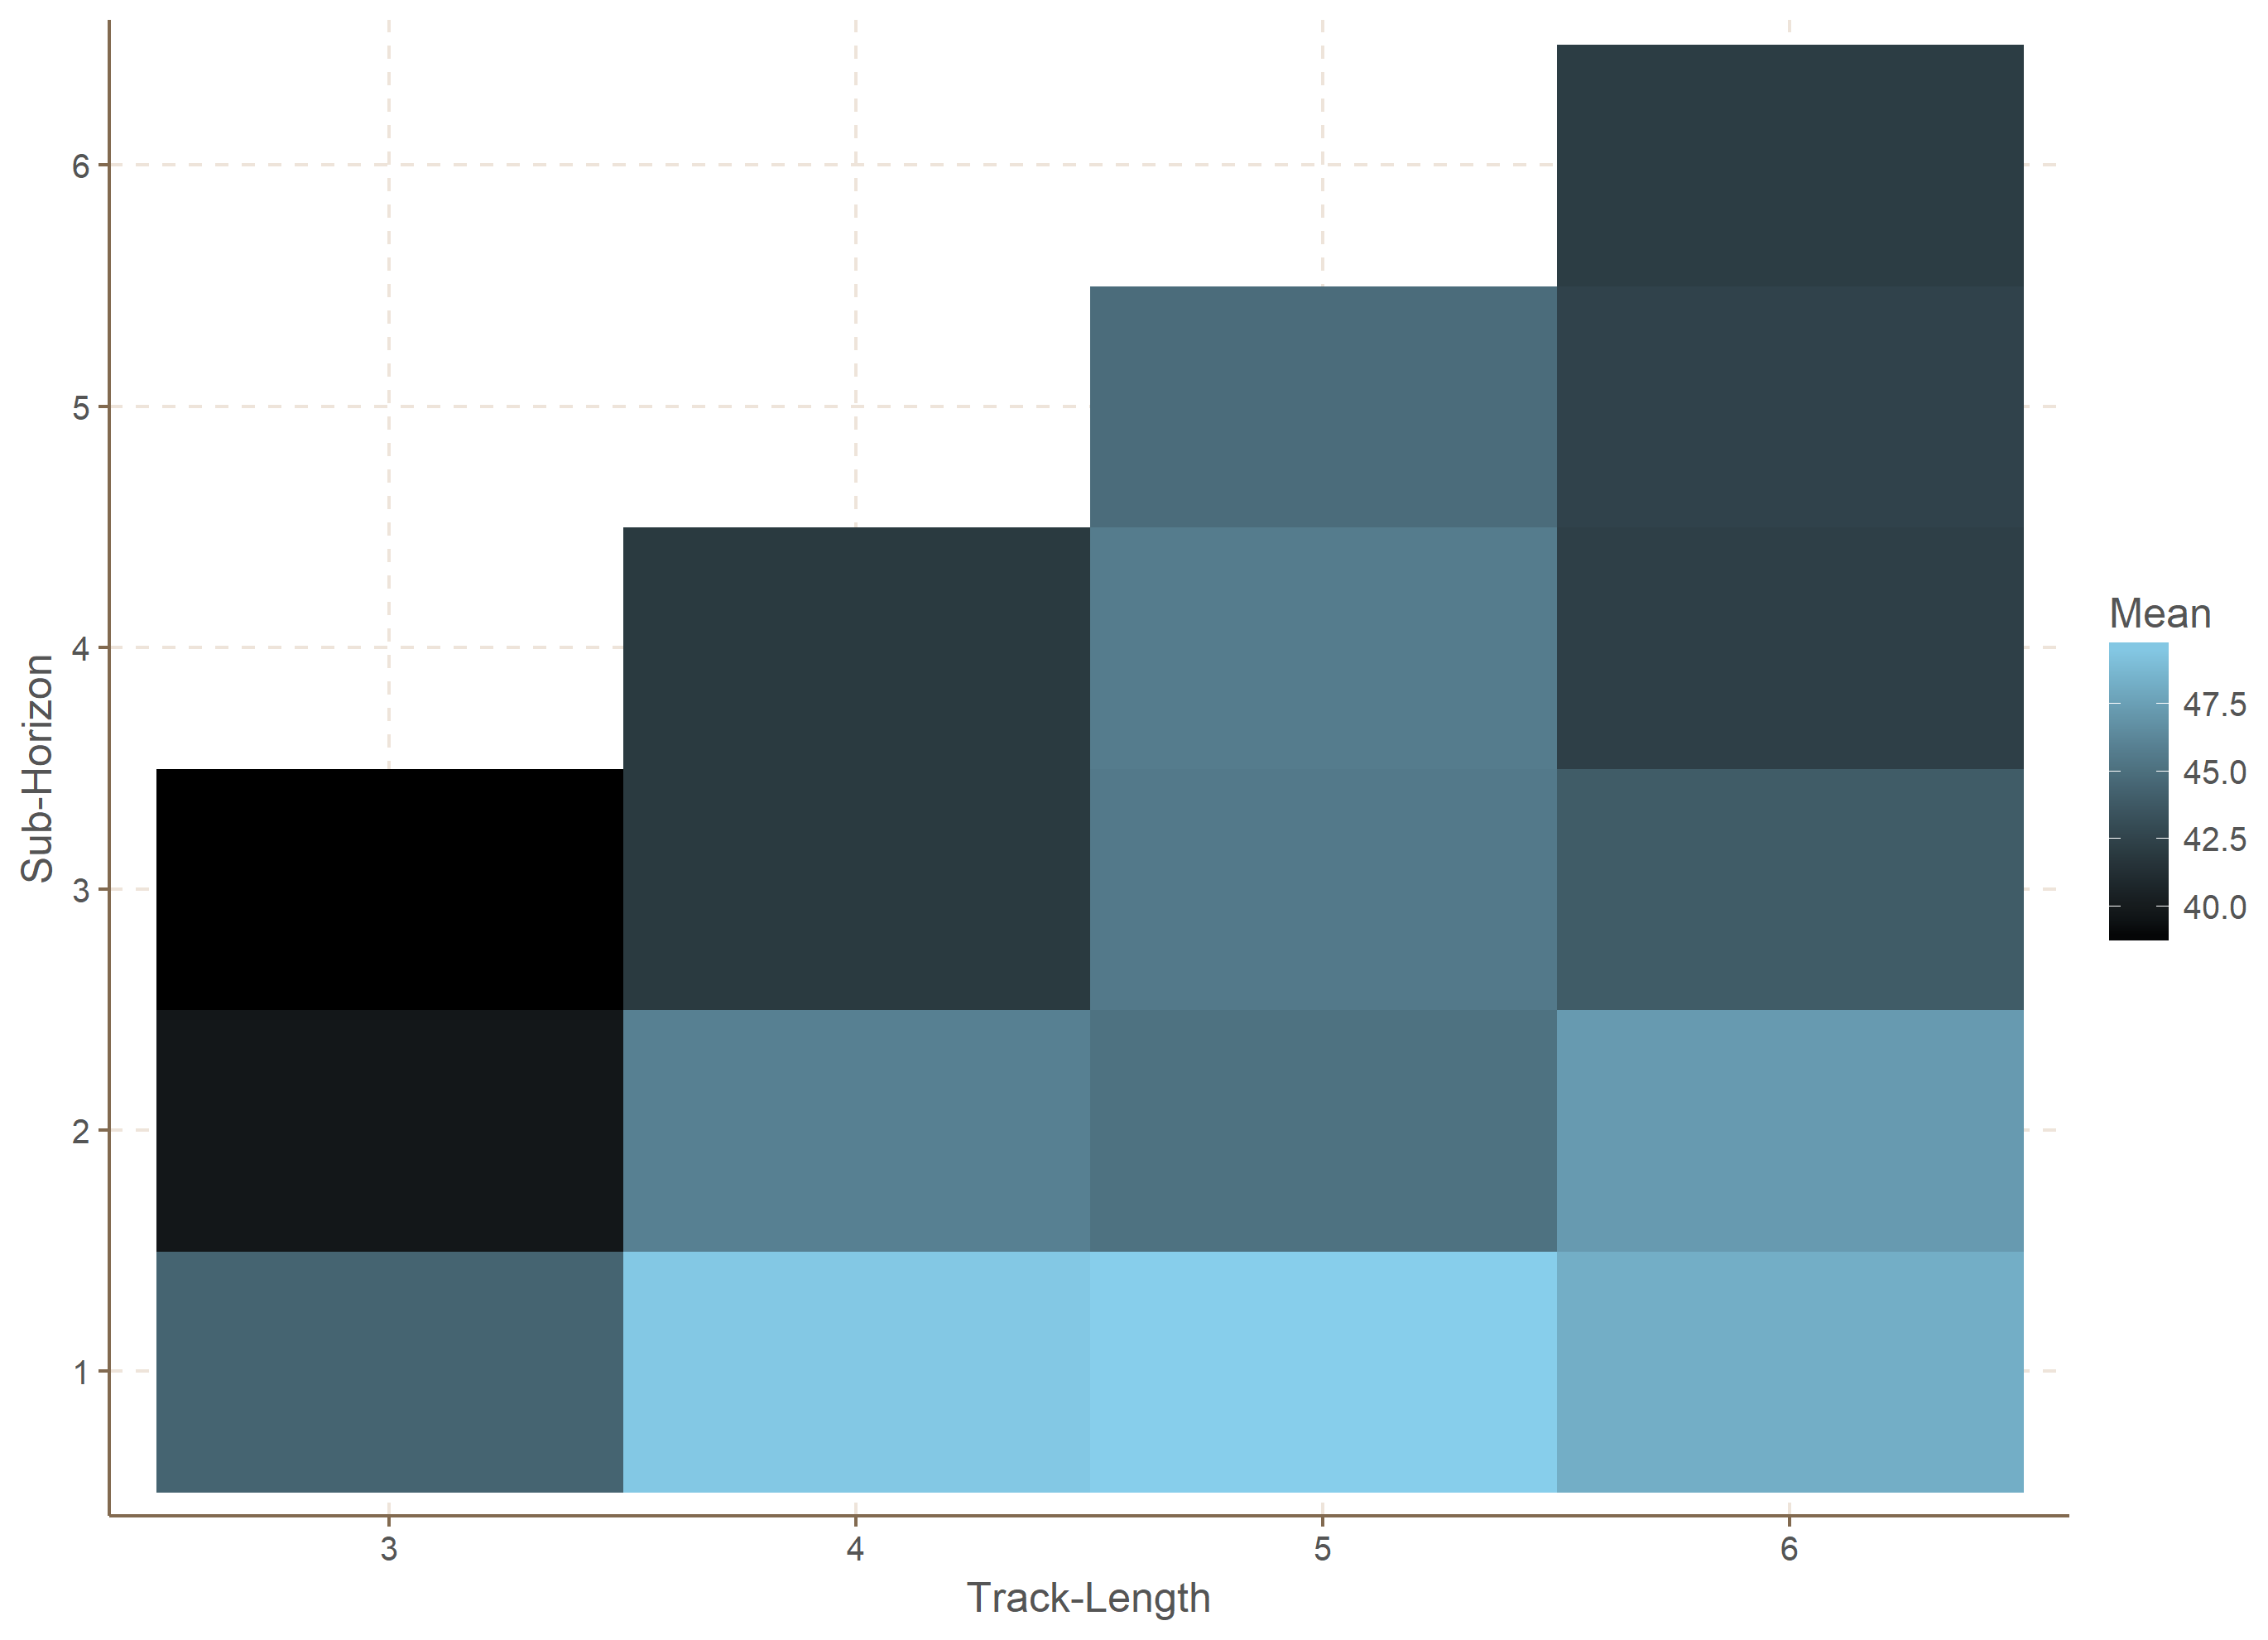
\includegraphics[scale=0.5]{fig/chapter_6/pen_4.png}
    \caption{Performance with changing sub-horizon and track-length and penalty, $R$, set to 4.}
\label{fig:pen_4}    
\end{figure}

Figure \ref{fig:pen_4} displays the results when considering track-lengths from 3-6 gameweeks as well as sub-horizons from 1-6 gameweeks.  Moreover, Table \ref{tab:pen_4_ill_trans} provides the numerical values of the combinations in Figure \ref{fig:pen_4} with the 10 highest means as well as average weekly penalized transfers made for these combinations.




\begin{table}[H]
\centering
\begin{tabular}{|l|l|l|l|c|}
\hline
Sub-horizon & Track-length & Objective Value & Mean & Penalized transfers \\
\hline
1       & 5          & 1644             & 49.82 & 1.48       \\
1       & 4          & 1684             & 49.53 & 1.88       \\
1       & 6          & 1544             & 48.25 & 1.34       \\
2       & 6          & 1513             & 47.28 & 2.09       \\
2       & 4          & 1562             & 45.94 & 2.74       \\
4       & 5          & 1509             & 45.73 & 2.88       \\
3       & 5          & 1504             & 45.58 & 2.70       \\
2       & 5          & 1491             & 45.18 & 2.55       \\
5       & 5          & 1481             & 44.88 & 3.00       \\
1       & 3          & 1555             & 44.43 & 2.63       \\
\hline
\end{tabular}
\caption{The 10 best combinations of track-lengths and sub-horizons.}
\label{tab:pen_4_ill_trans}
\end{table}


As observed in Figure \ref{fig:pen_4} and Table \ref{tab:pen_4_ill_trans}, the model reaches its best performances with a sub-horizon of 1 gameweek combined with track-lengths between 4-6 gameweeks. However, obtaining a weekly mean of 49.82 points would only have been sufficient enough to reach the top 35th percentile in the overall rankings. From Table \ref{tab:pen_4_ill_trans}, it is apparent that the model performs many penalized transfers. In general, making 1.5 penalized transfers on average each gameweek would penalize $1.5\cdot4\cdot38 = 228$ points, and have a huge impact on the overall rankings. Moreover, according to Table \ref{tab:pen_4_ill_trans}, the performances generally increases as the number of penalized transfers decreases. Consequently, in the following we investigate how regulations on the penalty parameter affects the results. This violates the game rules of FPL, and is in reality only a compensation for inaccurate forecasts. However, as we seek to maximize performance of the model, it is worth investigating. 


\subsubsection{Model run with different penalties}

To set values for the parameters penalty, track-length and sub-horizon, different combinations are tested on the 2016/2017 season. Figure \ref{Parameter_choice} provides an overview of how the mean value of points for the entire 2016/2017 season changes with different track-lengths, sub-horizons and penalty terms. Moreover, Table \ref{tab:top_10} provides the numerical values from the best 10 combinations in Figure \ref{Parameter_choice}.


\newpar

\begin{comment}
\textit{Avsnittet ovenfor må skrives mer utfyllende og inneholde mer diskusjon. Spesielt fra setningen "Frist, a sub-horizon of 3-4..." og utover. Viktige punker å få med: at dette er kun testet på en sesong og derfor må alt bli tatt med en klype salt. Man vil ikke teste for mer enn forecasting horizon på 6, siden da har man så få datapunker å basere seg på at det blir unfair å sammenlikne dens resultater med forecasting horizon på f.feks 2. Det skrives at sub-horizon på 3-4 ser ideell ut, men hvorfor? Det må skrives.}
\end{comment}


\begin{figure}[H]
    \centering
    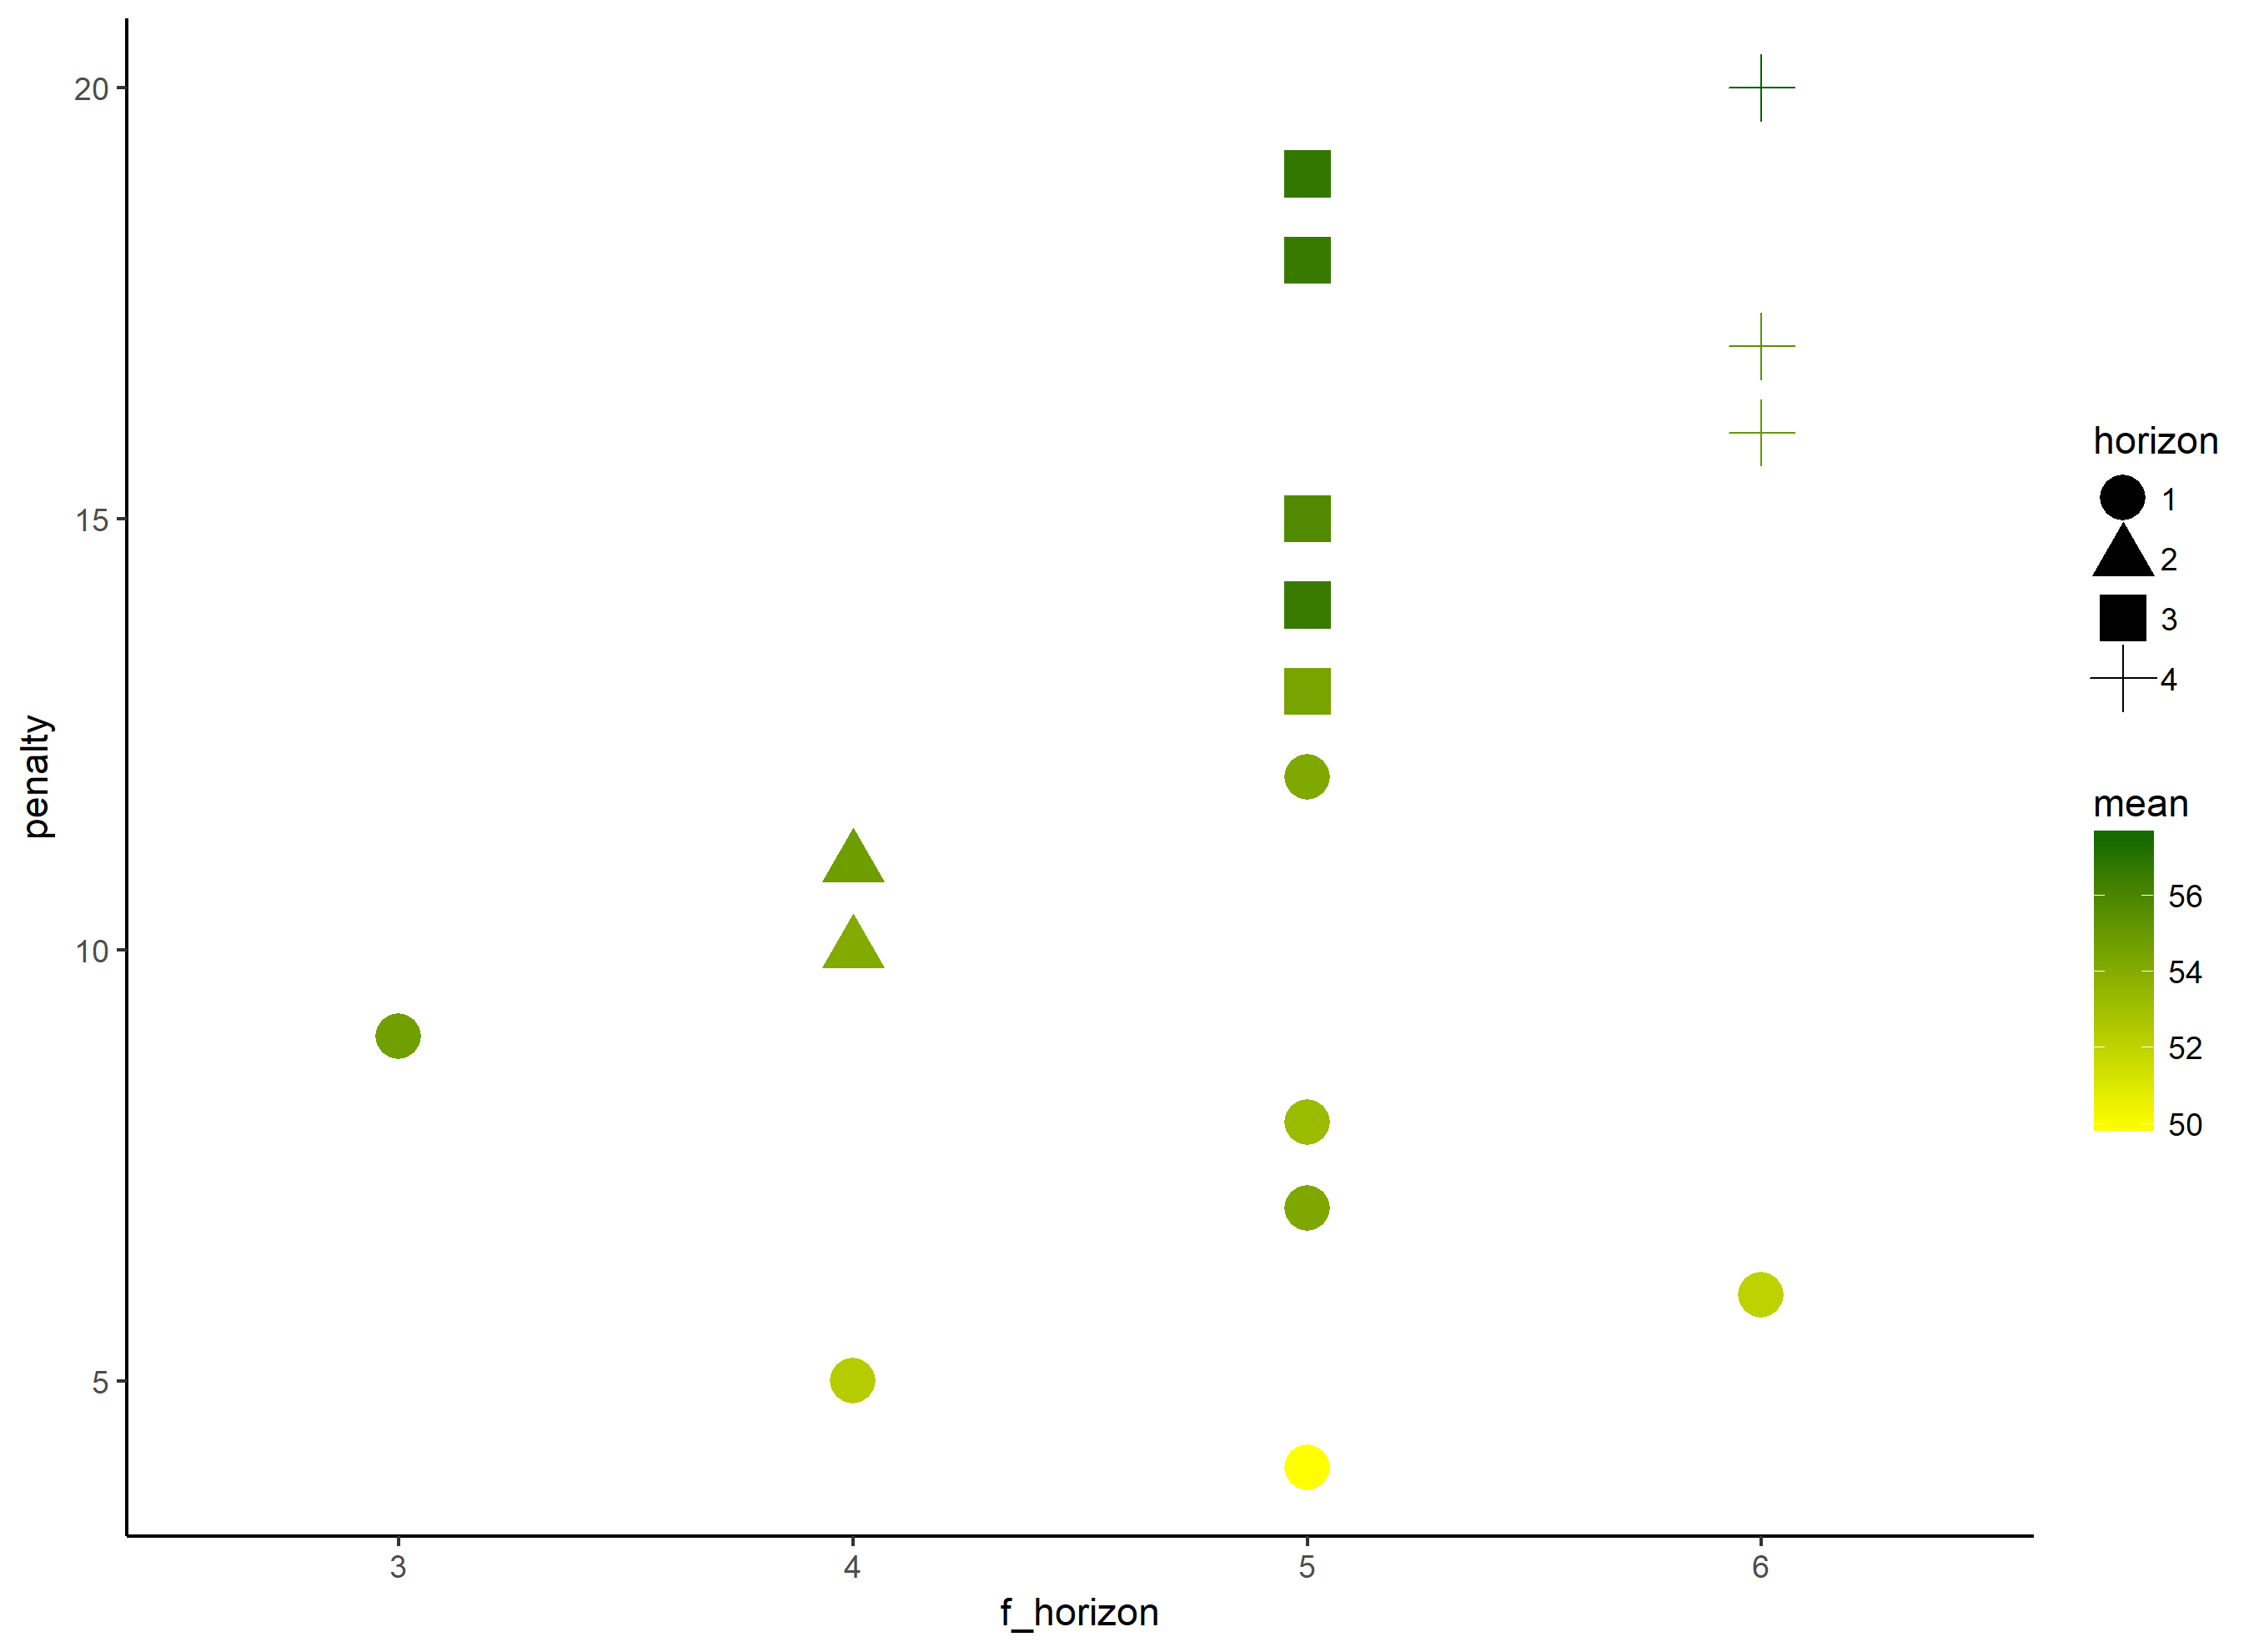
\includegraphics[scale=0.45]{fig/chapter_6/paramter_choice.png}
    \caption{Performance with different penalty term, sub-horizons and track-lengths.}
\label{Parameter_choice}    
\end{figure}

In Figure \ref{Parameter_choice}, only the best run (maximum mean) for each different penalty value from 3-20 is plotted. According to Figure \ref{Parameter_choice} and Table \ref{tab:top_10}, sub-horizons of 3-4 gameweeks appear to be ideal, as they provide the combinations with the highest mean performances. Furthermore, penalties in the range of 14-20 yield the best results. As for the track-lengths, values of 5 and 6 gameweeks are clearly optimal. However, the latter is not unexpected due to the bias in player selection. 

\begin{table}[H]
\centering
\begin{tabular}{|l|l|l|l|l|}
\hline
Penalty & Sub-horizon & Track-Length & Total Points & Mean  \\
\hline
20      & 4       & 6                & 1851         & 57.84 \\
20      & 4       & 5                & 1899         & 57.55 \\
19      & 3       & 5                & 1875         & 56.82 \\
18      & 3       & 5                & 1869         & 56.64 \\
14      & 3       & 5                & 1868         & 56.61 \\
18      & 4       & 6                & 1808         & 56.50 \\
19      & 4       & 6                & 1806         & 56.44 \\
20      & 3       & 5                & 1860         & 56.36 \\
20      & 5       & 5                & 1851         & 56.09 \\
18      & 6       & 6                & 1793         & 56.03 \\
\hline
\end{tabular}
\caption{The 10 best combinations of parameters.}
\label{tab:top_10}
\end{table}


Figure \ref{fig:fixed_f_hor} and Table \ref{tab:top_5} display the best combinations when the track-length is held fixed for 3-6 gameweeks. Clearly, track-lengths of 5 and 6 gameweeks outperform those of 3 and 4 gameweeks based on mean performance. Moreover, Table \ref{tab:top_10} shows that a track-length of 6 gameweeks combined with a sub-horizon of 4 gameweeks and a penalty term of 20 yields the highest mean for the 2016/2017 season. However, the next 4 highest means are achieved with a track-length of 5 gameweeks. Considering this, combined with the fact that an increasing track-length yield biased player predictions, we find it appropriate to select 5 gameweeks as the optimal track-length for the 2017/2018 season. Additionally, according to Figure \ref{fig:fixed_f_hor} an sub-horizon of 3 or 4 gameweeks is optimal. Combined with a track-length of 5, a sub-horizon of 3 gameweeks generally performs better than that of 4 gameweeks. Therefore, we find it convenient to set the sub-horizon to 3 gameweeks when applying the Modified Average approach for the 2017/2018 season. Finally, Figure \ref{fig:fixed_f_hor} illustrates that relatively high penalty terms yield the best means for the 2016/2017 season, with penalty terms ranging from 14-20. However, from Table \ref{tab:top_10} it is apparent that in combination with a track-length of 5 and sub-horizon of 3, the best penalty term is 14-19. Also, from Table \ref{tab:top_5} it is clear that the penalty term is considerably lower for the best combinations with a track-length of 3 and 4. Taken all this into consideration, we have decided on a penalty term, $R$, of 16.


\begin{figure}[H]
    \centering
    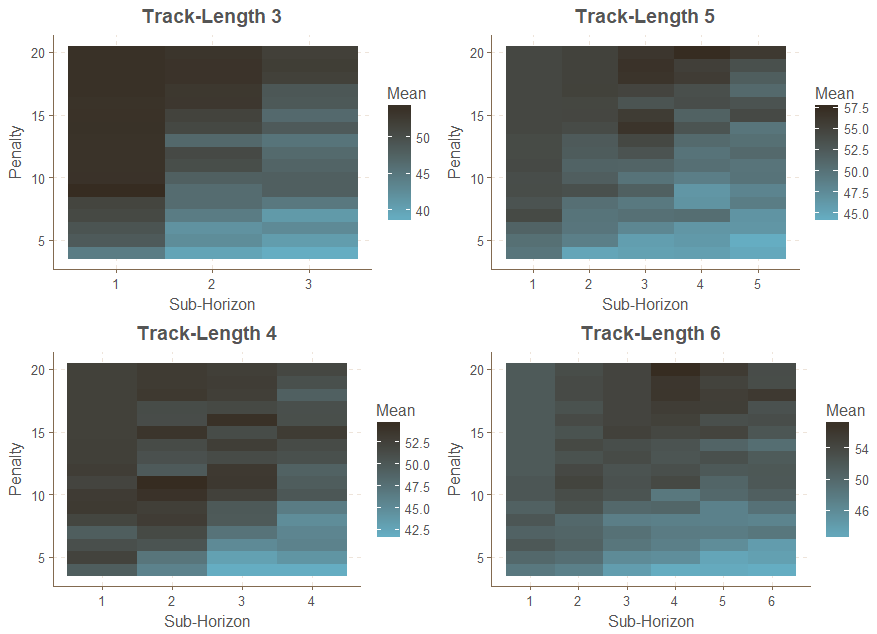
\includegraphics[scale=0.55]{fig/chapter_6/parameter_choice_fixed_f_hor.png}
    \caption{Performance with different penalty term, sub-horizons, but fixed track-lengths.}
\label{fig:fixed_f_hor}    
\end{figure}

\begin{table}[H]
\centering
\begin{tabular}{|l|l|l|l|l|}
\hline
Penalty & Horizon & Forecast Horizon & Total Points & Mean  \\
\hline
9       & 1       & 3                & 1914         & 54.69 \\
11      & 2       & 4                & 1863         & 54.79 \\
20      & 4       & 5                & 1899         & 57.55 \\
20      & 4       & 6                & 1851         & 57.84 \\
\hline
\end{tabular}
\caption{The best combinations for each track-length.}
\label{tab:top_5}
\end{table}


\newpar
To summarize the discussion above, we have chosen to run the Modified Average approach on the 2017/2018 season using the following parameters:

\begin{table}[H]
    \centering
    \begin{tabular}{|c|c|}
    \hline
    Parameters      &   Choices \\
    \hline
    Sub-horizon     &   3 gameweeks \\
    Track-length    &   5 gameweeks \\ 
    $R$             &   16 \\ 
    \hline
    \end{tabular}
\end{table}

\subsection{Regression}\label{exp_setup_reg}

\subsubsection{Variables}

As mentioned in Section \ref{exp_setup_data}, where it is reasonable, data are set equal to the last gameweeks of the 2016/2017 season. This is for instance the case for \textit{goals} and \textit{assists}. For \textit{transfers in} and \textit{transfers out}, however, this is not a sensible approach, as human manager do not base their transfer-decisions with the upcoming season in mind. Therefore, these values are set equal to 0 in the first gameweek. The variables \textit{saves} and \textit{penalty saves} are only defined for goalkeepers, and are thus only considered for goalkeepers.

\subsubsection{Categorization based on Position}

As outlined in Section \ref{Sol_approach_regression}, we have decided to separate the players based on their positions. To substantiate this decision, a visual assessment is undertaken. The analysis is done for the final gameweek of the 2016/2017 season, as it constitutes the training set used. First, Figure \ref{fig:cluster_plots} displays a box-plot of the total points for each different position. The different positions appear to exhibit some differing characteristics. The variance seems larger for midfielders and forwards than what it is for defenders and goalkeepers. Further, defenders and goalkeepers have the highest median scores, while the most positive outliers are found among midfielders and forwards. Secondly, the figure shows how total points are associated with the variables \textit{clean sheets}, goals and assists for different positions. It is clear that goals and assists are not contributing a lot in terms of total points for goalkeepers, but are important for midfielders and forwards. Figure \ref{fig:cluster_plots} also manifest that clean sheets are important for goalkeepers and defenders in order to earn a high point score.

\begin{figure}[H]
    \centering
    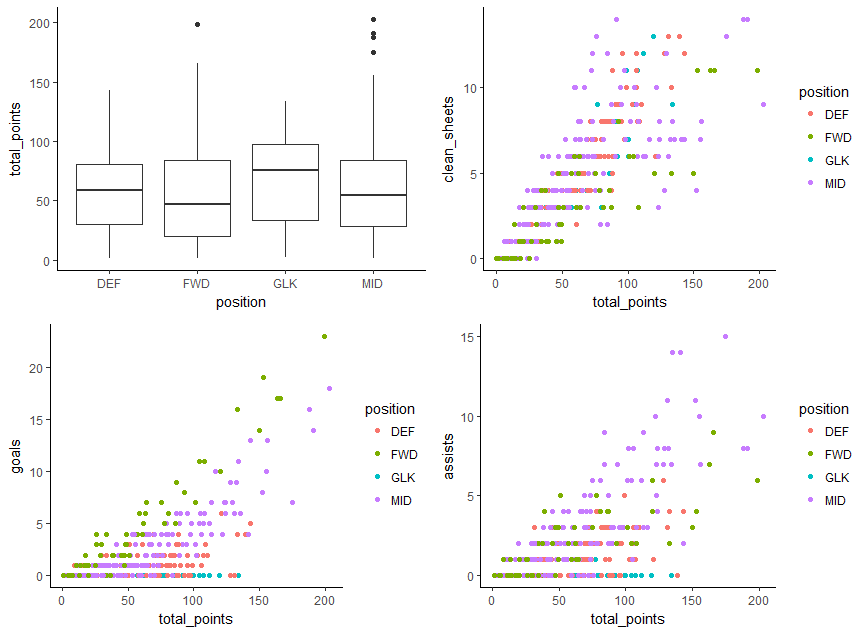
\includegraphics[scale=0.55]{fig/chapter_6/cluster_plots.png}
    \caption{Plots substantiating the decision of separating the players based on position.}
\label{fig:cluster_plots}    
\end{figure}


\subsubsection{Time Series of Points}

In order to determine if one should treat the points a player obtains as a time series (i.e the effect of form), the Durbin-Watson test and the Ljung-Box test with lag 1-5 for autocorrelation are performed. Table \ref{tab:auto_tests} presents the results of the tests. Based on the results, 75\%-95\% of the players exhibit insignificant autocorrelation in their time-series of points at a significance level of 10 \%, and 80\%-99\% at significance level 5\%. The results indicate no autocorrelation effects. However, this result should be interpreted carefully as individual players may still display a time-dependency in points obtained. Regardless, we have decided to neglect time-series effects in the regression. That is, the variable \textit{previous points} is excluded from consideration. The methodology works as a complement to the Modified Average method.

\begin{table}[H]
\centering
\begin{tabular}{|l|c|c|}
\hline
Test            & \% significance level 10\% & \% significance level 5\% \\
\hline
Durbin-Watson   & 94 \% & 99 \%                                            \\
Ljung-Box lag 1 & 76 \% & 84 \%                                            \\
Ljung-Box lag 2 & 76 \% & 81 \%                                            \\
Ljung-Box lag 3 & 78 \% & 84 \%                                            \\
Ljung-Box lag 4 & 80 \% & 84 \%                                           \\
Ljung-Box lag 5 & 81 \% & 85 \%                
\\
\hline
\end{tabular}
\caption{Summary of percentage of players with insignificant autocorrelation for different tests and significance levels.}
\label{tab:auto_tests}
\end{table}

\subsubsection{Variable Selection}

As described in Section \ref{Sol_approach_regression}, lasso regression with \textit{k}-fold cross validation is performed in order to conduct a variable selection. Data from the entire 2016/2017 season is used, and separated into $\textit{k}=10$ folds for the cross validation. In Figure \ref{fig:lasso_all}, a plot of (average \textit{k}-fold) MSE against values of log($\lambda$) for each position is presented. Note that in each plot there are 2 dotted vertical lines. The leftmost line marks the log($\lambda$)-value with lowest MSE. The rightmost marks the log($\lambda$)-value with one standard deviation higher MSE than the lowest MSE. Furthermore, the numbers in the top of the plot indicate the number of variables included for each value of log($\lambda$). The reason why the number of variables may exceed the number of variables presented in Section \ref{Sol_approach_regression}, is that a dummy-variable is introduced for each level of a categorical variable. That is, the variables \textit{team} and \textit{opponent} will be treated as 20 different variables each as there are 20 teams (levels) in the English Premier League. If only a few of the dummy-variables are selected by the lasso-regression, the variable associated with them is excluded from consideration. Similarly, if all except a few dummy-variables are selected, all levels are included. That is, some levels are included even if they are not selected by the lasso regression.

\newpar

\begin{figure}[H]
    \centering
    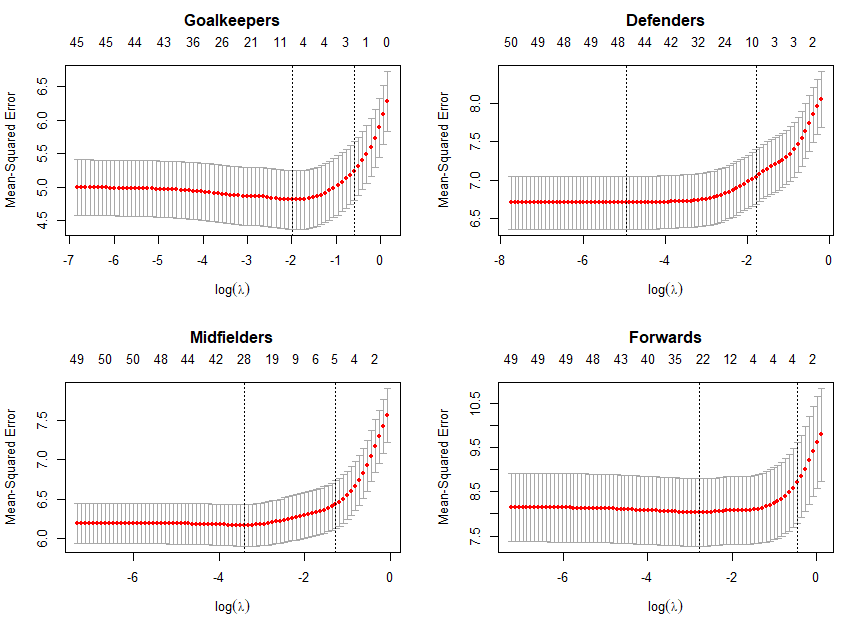
\includegraphics[scale=0.55]{fig/chapter_6/lasso_all.png}
    \caption{\textit{k}-fold cross validated MSE for different values of log($\lambda$) for the different positions.}
\label{fig:lasso_all}    
\end{figure}

\subsubsection{Model Selection}
For each position, a linear regression model is fitted based on the variables selected. In the following, a presentation of the selected variables and a summary of each model is presented. The $\beta$-coefficients presented are computed before the 2017/2018 season. Note that even though the variables are the same throughout the season, the $\beta$-coefficients are subject to change, as each model is refitted every gameweek when new data becomes available. Even if team or opponent are selected, they are not presented in the summary, as they would require 20 variables each.

\newpar

\subsubsection{Goalkeepers}

As evident from Figure \ref{fig:cluster_plots},f no goalkeepers scored a goal in the 2016/2017 English Premier League season, and only one assist was provided by a goalkeeper. Therefore, we have decided not to consider these explanatory variables when performing the variable selection for goalkeepers. Figure \ref{fig:lasso_all} shows that for the lowest MSE, 6 variables are included in the model. With only 6 variables present, the possibility of overfitting is limited. Therefore, all the variables associated with this log($\lambda$)-value are considered. However, one of them were related to a team, and another to an opponent. As only 1 of 20 variables for team and opponent were included, both team and opponent are excluded from consideration. In Table \ref{tab:coef_GLK} a summary of a regression fitted on the selected variables is presented. All variables have a sign consistent with their intuitive interpretation. The p-values indicate that all variables are significant. 

\begin{table}[H]
\centering
\begin{tabular}{|l|l|l|l|l|}
\hline
Variable     & Coefficient ($\beta$) & Std. Error & t-value & p-value \\ \hline
(Intercept)  & -3,35E+00    & 7,1E-01    & -4,7    & 2,4E-06               \\
Cost         & 8,33E-07 & 1,6E-07    & 5,3     & 1,4E-07               \\
Transfers in & 4,50E-05 & 7,0E-06    & 6,4     & 2,3E-10               \\
Minutes      & 1,12E-02 & 2,0E-03    & 5,5     & 4,0E-08               \\
Saves        & 1,76E-02 & 2,8E-03    & 6,4     & 2,4E-10
\\
\hline
\end{tabular}
\caption{Summary of the linear regression for goalkeepers.}
\label{tab:coef_GLK}
\end{table}

\begin{table}[H]
\centering
\begin{tabular}{|l|l|}
\hline
Variable     & Value   \\ \hline
Cost         & 5.5 $\cdot$ $10^6$ \\
Transfers in & 13 884   \\
Minutes      & 90      \\
Saves        & 20     \\
\hline
\end{tabular}
\caption{Variables for Petr Cech for gameweek 9.}
\label{tab:var_petr}
\end{table}

Table \ref{tab:var_petr} shows the cost, transfers in, minutes and saves of Petr Cech ahead of gameweek 9 in the 2017/2018 season. His expected points could be computed as:

\begin{equation*}
    -3.35 + 8.33\cdot10^{-7}\cdot5.5\cdot10^6 + 4.5\cdot10^{-5}\cdot13 884 + 1.12\cdot10^{-2}\cdot90 + 20\cdot1.76\cdot10^{-2} \approx 3.2
\end{equation*}

Note that the illustration does not capture the fact that the $\beta$ are subject to change due to new available information and refitting of the model.


\subsubsection{Defenders}

As evident from Figure \ref{fig:cluster_plots}, defenders frequently provide assists and goals. Therefore, these variables are not excluded when performing the variable selection for defenders. From Figure \ref{fig:lasso_all} it is apparent that the model with the lowest MSE value includes approximately 47 variables, while the model one standard deviation away (indicated by the rightmost dotted line), includes 10 variables for defenders. By taking overfitting into consideration, the model corresponding to the log($\lambda$)-value with MSE one standard deviation higher than the minimum MSE is chosen.

\newpar

None of the variables associated with team were selected, but 4 of the variables associated with opponent were included. Therefore, team is excluded from the linear regression, but opponent is not. In Table \ref{tab:coef_DEF} a summary of the selected variables can be found. Note that the coefficient corresponding to the variable \textit{home/away} is multiplied by 1 if a player plays at home, and 0 otherwise. Thus, the signs in front of all coefficients except the variable \textit{yellow cards} make intuitive sense. A justification for the positive sign in front of yellow cards is perhaps that players receiving many yellow cards are also frequently involved in matches, thus earning points from other activities. It is worth noting that yellow cards is the variable in Table \ref{tab:coef_DEF} with lowest p-value, even if they are all significant at a significance level of 0.01.

\begin{table}[H]
\centering
\begin{tabular}{|l|l|l|l|l|}
\hline
Variable      & Coefficient ($\beta$) & Std. Error & t-value & p-value \\ \hline
(Intercept)   & -3,5E+00     & 3,9E-01    & -9,00    & 3,4E-19 \\
Cost          & 7,9E-07      & 7,4E-08    & 10,7    & 2,4E-26 \\
Transfers in  & 2,7E-05      & 3,2E-06    & 8,54     & 1,9E-17 \\
Transfers out & -1,9E-05     & 3,1E-06    & -6,10    & 1,1E-09 \\
Home/Away     & 3,9E-01      & 8,5E-02    & 4,54     & 5,8E-06 \\
Minutes       & 1,2E-02      & 1,1E-03    & 11,2    & 1,3E-28 \\
Yellow Cards  & 7,9E-02      & 2,0E-02    & 3,88     & 1,1E-04 \\
\hline
\end{tabular}
\caption{Summary of the linear regression for Defenders.}
\label{tab:coef_DEF}
\end{table}


\subsubsection{Midfielders}
From Figure \ref{fig:lasso_all}, it is apparent that the model with the lowest MSE value includes 28 variables for midfielders, while the model one standard deviation away includes 5. We suspect that more than 5 variables can have a higher predictive power. Thus, we have decided to choose the model with 28 variables. A substantial amount of the levels corresponding to both team and opponents are included, so both variables are carried forward. The coefficients from the linear regression are presented in Table \ref{tab:coef_MID}. All signs in front of the coefficients are consistent with their intuitive interpretation. Furthermore, they are all significant at a significance level of 5\%.

\begin{table}[H]
\centering
\begin{tabular}{|l|l|l|l|l|}
\hline
Variable         & Coefficient ($\beta$)  & Std. Error & t value & p-value \\ \hline
(Intercept)      & -2,05E+00 & 3,0E-01    & -6,94   & 4,3E-12 \\
Cost             & 4,76E-07  & 3,6E-08    & 13,1   & 2,4E-38 \\
Transfers In     & 9,85E-06  & 1,4E-06    & 7,18    & 8,0E-13 \\
Transfers Out    & -8,03E-06 & 1,5E-06    & -5,47   & 4,8E-08 \\
Home/Away        & 2,82E-01  & 6,7E-02    & 4,19    & 2,9E-05 \\
Minutes          & 1,01E-02  & 9,5E-04    & 10,7   & 2,9E-26 \\
Goals            & 7,57E-02  & 2,2E-02    & 3,51    & 4,5E-04 \\
Penalties Missed & -3,98E-01 & 1,7E-01    & -2,31   & 2,1E-02 \\
Clean Sheets     & 6,78E-02  & 1,6E-02    & 4,21    & 2,6E-05 \\
Assists          & 5,23E-02  & 2,0E-02    & 2,61    & 9,1E-03 \\
\hline
\end{tabular}
\caption{Summary of the linear regression for midfielders.}
\label{tab:coef_MID}
\end{table}


\subsubsection{Forwards}
For forwards, the variable clean sheet is not taken into consideration. Forwards are not rewarded for clean sheets, and from Figure \ref{fig:cluster_plots} it is hard to spot a pattern between total points and clean sheets for forwards. The Figure \ref{fig:lasso_all} shows that for forwards, the model with the lowest MSE value includes 25 variables, while the model one standard deviation away includes 4. Again, we suspect that more than 4 variables have a higher predictive power, and hence the model with minimum MSE is selected. Enough levels of the variables team and opponent are included to make it justifiable to select them. The coefficients from the linear regression are presented in Table \ref{tab:coef_FWD}. All the signs in front of the coefficients appear consistent with their intuitive interpretation, except for the variable \textit{penalties missed}. This can perhaps stem from that fact that if a player misses a penalty, he might also frequently take the penalties for his team, thus earning points when he scores. Note however, that both home/away and penalties missed are insignificant in the linear regression model for a significance level of 5\%. Regardless, we have decided to include them, as they were initially selected by the lasso regression.

\begin{table}[H]
\centering
\begin{tabular}{|l|l|l|l|l|}
\hline
Variable         & Coefficient ($\beta$)  & Std. Error & t value & p-value \\ \hline
(Intercept)      & -1,75E+00 & 6,7E-01    & -2,62   & 9,0E-03 \\
Cost             & 3,89E-07  & 6,7E-08    & 5,79    & 8,4E-09 \\
Transfers In     & 1,39E-05  & 1,9E-06    & 7,24    & 6,8E-13 \\
Transfers Out    & -5,40E-06 & 1,8E-06    & -3,03   & 2,5E-03 \\
Home/Away        & 1,52E-01  & 1,4E-01    & 1,10    & 2,7E-01 \\
Minutes          & 9,02E-03  & 2,3E-03    & 3,99    & 6,9E-05 \\
Goals            & 6,54E-02  & 2,6E-02    & 2,55    & 1,1E-02 \\
Penalties Missed & 5,52E-01  & 3,0E-01    & 1,87    & 6,2E-02 \\
\hline
\end{tabular}
\caption{Summary of the linear regression for forwards.}
\label{tab:coef_FWD}
\end{table}

\subsubsection{Remarks}

An interesting observation from the variable selection is that team and clean sheets are not selected for goalkeepers or defenders. Forcing the variable into the model could be an interesting approach in order to investigate what difference it makes, but is not considered in this thesis. Using total sums, for instance for saves, goals and assists, constitute a drawback in the sense that observations are quite similar for all players in the first gameweeks. One way to account for this is to include values from last season in more than the first gameweek. This approach would, however, complicate the process of including players with a lack of data even further. Another approach would be to only fit the model on data from the first gameweeks of previous seasons. However, that would be more sensible if data for multiple seasons were used in the training set.

\newpar

Since we only have data for one season to train the model, we have considered it infeasible to also perform a parameter-study. Therefore, we have set the penalty term to 4, as stated in the game-rules. The sub-horizon is set to equal to the sub-horizon in the Modified Average approach, namely to 3.

\subsection{Odds}

In order to obtain necessary data, we have cooperated with Sportradar, a Norwegian company providing data for bookmakers. Sportradar delivers odds and probabilities of several sports events, including English Premier League. They have provided us with all the necessary probabilities, including result outcomes for each Premier League match as well as individual probabilities such as goals scored, assists given and yellow cards achieved. These data made all the computational work a lot easier, as Sportradar exported structured excel files containing all the necessary data. Sportsradar provided us with data for the 30 first gameweeks of the 2017/2018 season. However, data were lacking for some matches in gameweek 7 and 13. This is important to keep in mind for the computational study in Chapter \ref{chapter_computational_study}.

\newpar

Compared to the other two solution approaches, the player list is limited when calculating expected points using odds probabilities. The data from Sportradar was delivered post-season, which has affected the player list. Players that has been transferred or lend to other clubs during the 2017/2018 season are not considered. This is due to the fact that these players are no longer listed in Sportradar's database of Premier League players. In general, the reduced player list will not affect the results of the model, as the players that are lend out are typically lend to clubs in the English Championship division. Hence, these players were not consider good enough to contribute for the teams in the Premier League. However, some of the transfers might have an impact on the results. For instance, players like Philippe Coutinho and Michy Batshuayi are players that contributed with fantasy points in the first half of the season. Unfortunately, these players are not considered when using the odds approach, which is considered as a drawback of the approach. 

\newpar
As odds are primarily available for fixtures in the near future, primarily for the upcoming gameweek, the forecast method using odds is further limited. In our case, we only have odds available one gameweek ahead. Hence, the sub-horizon in the optimization model is forced to be one gameweek. Compared to the other suggested methods, this is considered a drawback. Furthermore, the penalty term, $R$, is set to 4 as stated in the game rules. 


\section{Gamechips} \label{exp_setup_gamechips}

The game chips are played according to the solution framework suggested in Section \ref{Ch.5_Game_chips}. By examining the fixtures list of this year's Premier League season, we have made the following decisions. The model is given the opportunity of playing the first Wildcard in gameweek 9. It can either choose to play it or disregard it for the first half of the season. Hence, the model is not given the opportunity to play the first Wildcard in any other gameweek. Further, the Triple Captain can only be played in gameweek 22, as this is the first double gameweek of the season. Moreover, we allow the Bench Boost to be played in the second double gameweek of the season, gameweek 34. Thus, the model is given the opportunity to play the second Wildcard in gameweek 33, preparing for the Bench Boost in the following gameweek. As we chose to play the Bench Boost in the double gameweek 34, we have chosen to play the Free Hit in a blank gameweek. We allow the model to play a Free Hit in gameweek 31, which is a blank gameweek, were only 8 teams are featured. 

\newpar

Notice that the decisions on when to play the gamechips are not fixed ahead of the season. However, they are incorporated as the fixture list is updated with regards to blank and double gameweeks. Hence, the gamechips are first considered when a double or blank gameweek arise in the sub-horizon. As stated in Section \ref{exp_setup_data}, we assume that the model knows the status of a gameweek as many gameweeks ahead as the length of the sub-horizon, i.e. 3 gameweeks beforehand. If this was not the case, the assumption could give the model an unfair advantage over human managers. However, this was never the case in the 2017/2018 season.


 
\section{Risk Handling} \label{exp_setup_Value_Variance}

\subsection{Variance in the proposed model}

In order to estimate the variance of each player and the correlation between players, their historical performances are considered. To obtain reliable estimations, data for the entire 2016/2017 season is used. Therefore, it is impossible to also find a suitable variance threshold using data on the 2016/2017 season. As a consequence, we have decided to do an ex-post analysis of how the risk handling constraints effect the solution obtained in the 2017/2018 season, thus providing a basis for future research and models.

\subsection{Player Variance Estimation}

Each player's variance is calculated as the empirical variance in points obtained. All available data from the 2016/2017 and the 2017/2018 season are used. That is, for gameweek 10 of the 2017/2018, data from all rounds of the 2016/2017 as well as the first nine gameweeks of the 2017/2018 season is used. This method of estimation is sensible for the Modified Average method, as it does not aim to explain any of the variance. However, for the regression based model, the explanatory variables are assumed to explain some of the variance. Therefore it would be more suitable to estimate the variance based on the variance of the residuals. In the study conducted in Chapter \ref{chapter_computational_study}, only the Modified Average method is considered. 

\newpar

\subsubsection{Special cases}

\textit{Lack of historical data}
\newline
As previously discussed, complete historical data will not be available for all players for reasons such as promotion or transfers. If only one data point is available for a player (i.e he has only played one match), it is impossible to calculate his variance. In these cases, the variance is set equal to the average variance of all other players. It is worth noting that this will only be an issue for one match, as more than one data point will exist afterwards. The lack of data points are obviously a limitation of the accuracy of the variance estimation, and constitutes a significant source of uncertainty. As risk handling is a method undertaken in order to reduce overall risk, another approach might consider only picking players with a history of for example 10 gameweeks. \newpar

\textit{Zero Variance}
\newline
Some players have empirical variance equal to 0. For instance, players that have never played, can still be selected. Thus, they may have low number of expected points and a low cost. These players might be interesting to select in order to fulfill the selected squad constraints. However, it is not desirable to set their variance to 0, as the future performance is not deterministic. That is, they are \textit{not} analogous to the risk-free asset in a portfolio optimization setting. Therefore, their variance is set equal the lowest non-zero variance obtained by other players.

\subsection{Correlation Estimation}

In order to determine the correlation between two players on the same or opposing teams, historical data for the 2016/2017 season is considered. Note that data is aggregated such that only the correlation coefficient between different positions overall is considered. It is not calculated between individual players or teams. Therefore, the correlation between players in the same position in the same team is set equal to 1. The correlation between players that are not on the same team, nor facing each other in a game-week, is assumed to be 0.

\newpar

Table \ref{tab:cor_team} and Table \ref{tab:cor_opp} show the correlation coefficient between different positions. The tables also include the p-value from a Pearson's Product-Moment Correlation test where the alternative hypothesis is a correlation not equal to 0, for players of the same and opposing teams, respectively. In the cases where the correlation is not significant, GLK FWD and DEF FWD of the same teams and GLK GLK of opposing teams, the correlation coefficient is set equal to 0. For the rest, the correlation coefficients , $\rho$, presented in the tables are used.

\begin{table}[H]
\centering
\begin{tabular}{|l|l|l|l|}
\hline
Position & Position & $\rho$    & p-value  \\
\hline
GLK      & DEF      & 0.689  & 2.20 E-16 \\
GLK      & MID      & 0.274  & 1.24 E-10 \\
GLK      & FWD      & 0.0288 & 0.519    \\
DEF      & MID      & 0.368  & 2.20 E-16 \\
DEF      & FWD      & 0.0578 & 0.176    \\
MID      & FWD      & 0.238  & 1.72 E-08 \\
\hline
\end{tabular}
\caption{Correlation coefficient $\rho$ and p-value from significance test for the correlation between players of the same team.}
\label{tab:cor_team}
\end{table}

\begin{table}[H]
\centering
\begin{tabular}{|l|l|l|l|}
\hline
Position & Position & $\rho$    & p-value  \\
\hline
GLK      & GLK      & 0.0162 & 0.759    \\
GLK      & DEF      & -0.106 & 0.0374   \\
GLK      & MID      & -0.312 & 2.78E-10 \\
GLK      & FWD      & -0.336 & 3.85E-16 \\
DEF      & DEF      & -0.319 & 2.35E-11 \\
DEF      & MID      & -0.447 & 2.20E-16 \\
DEF      & FWD      & -0.292 & 3.35E-09 \\
MID      & MID      & -0.254 & 1.00E-07 \\
MID      & FWD      & -0.136 & 0.00632 \\
FWD      & FWD      & -0.119 & 0.0218  \\
\hline
\end{tabular}
\caption{Correlation coefficient $\rho$ and p-value from significance test for the correlation between players of opposing teams.}
\label{tab:cor_opp}
\end{table}